\documentclass[pdflatex,sn-vancouver-num]{sn-jnl}

%
% Set to \finalsubmissiontrue when compiling on a system without Inkscape and/or
% -shell-escape (e.g. most cloud/journal LaTeX services). Figures are then taken
% from pre-rendered PDFs instead of being converted from SVG on the fly; run
% convert-svgs-to-pdf.sh once beforehand to produce them.
\newif\iffinalsubmission
\finalsubmissionfalse

\usepackage{graphicx}%
\iffinalsubmission\else\usepackage{svg}%
\fi
\usepackage{multirow}%
\usepackage{amsmath,amssymb,amsfonts}%
\usepackage{amsthm}%
\newtheorem{proposition}{Proposition}%
\usepackage{mathrsfs}%
\usepackage[title]{appendix}%
\usepackage{xcolor}%
\usepackage{textcomp}%
\usepackage{manyfoot}%
\usepackage{booktabs}%
\usepackage{algorithm}%
\usepackage{algorithmicx}%
\usepackage{algpseudocode}%
\usepackage{listings}%
%\usepackage{qtree}
\usepackage{tikz-qtree}
%\usepackage{paper}
%
%\usepackage{xstring}
\usepackage{csquotes}
\usepackage{pgfplots}
\usepgfplotslibrary{fillbetween}
\usepgfplotslibrary{statistics}

\usepackage{csvsimple}
\usepackage{listings}
\usepackage{siunitx}
%\usepackage{multirow}
%\pgfplotsset{compat=1.5}
%\bibliographystyle{bibliography}
%\usepgfplotslibrary{external}
%\tikzexternalize
\usepackage{xr}
\usepackage{todonotes}
\externaldocument{supplements}

\usepackage{array}
\newcolumntype{L}[1]{>{\raggedright\let\newline\\\arraybackslash\hspace{0pt}}m{#1}}
\newcolumntype{C}[1]{>{\centering\let\newline\\\arraybackslash\hspace{0pt}}m{#1}}
\newcolumntype{R}[1]{>{\raggedleft\let\newline\\\arraybackslash\hspace{0pt}}m{#1}}

%
% Workaround for local / relative path problems in conjunction with reading csv file.
%
%\newcommand{\csvpath}{}

%
% Workaround for faster compile without scatter plots:
%
%\newif\ifscatter
%\scattertrue

%
% Includes an SVG figure produced by ft-db-exp2, e.g. \dbfig[width=12cm]{results/orthopox_ftsvgtaxtree}.
% Converts on the fly via Inkscape unless \finalsubmissiontrue, in which case a pre-rendered
% <name>.pdf next to the <name>.svg (see convert-svgs-to-pdf.sh) is used instead.
\newcommand{\dbfig}[2][]{%
\iffinalsubmission
\includegraphics[#1]{#2.pdf}%
\else
\includesvg[#1]{#2}%
\fi
}

%
% Draws a box plot of the relative k-mer distribution across rank intervals from a
% `kmerrankstats' CSV produced by ft-db-exp2, e.g.
%   \rankboxplot{results/tick-borne_kmerrankstatscsv.csv}
% One box per row of the CSV, so the plot follows the data: the boxes, their number and
% the tick labels are all read at compile time. The box spans the first and third quartile
% (columns `rel q1' and `rel q3') with the median (`rel median') as the middle line, and the
% whiskers are the Tukey whiskers (`rel whisker low' and `rel whisker high').
% As a side effect, \speciescount holds the underlying number of species (column
% `species count') so that it can be quoted in the caption.
% CSV files written before the whisker columns were added to KMerRankStatsCSVGoal lack the two
% whisker columns and have the remaining ones at lower indices. Such files are still accepted,
% detected by the absence of a 16th column, and are then drawn without whiskers. This fallback
% may be dropped once all CSV files under results/ have been regenerated.
% The optional argument is the plot's title, used for the (a)/(b) labels of a combined figure.
\newcommand{\rankboxplot}[2][]{%
\def\ranklabels{}%
\csvreader[separator=semicolon]{#2}{}%
{\xdef\speciescount{\ifcsname csvcolxvi\endcsname\csvcolix\else\csvcolvii\fi}%
 \xdef\nranks{\thecsvrow}%
 \xdef\ranklabels{\ifnum\thecsvrow=1\else\ranklabels,\fi{\csvcoli}}}%
\begin{tikzpicture}
\begin{axis}[
  title={#1}, title style={font=\footnotesize},
  boxplot/draw direction=y, ymin=-0.02, ymax=1.02,
  xmin=0.5, xmax=\nranks+0.5,
  xtick/.expanded={1,...,\nranks}, xticklabels/.expanded=\ranklabels,
  x tick label style={rotate=40, anchor=north east, font=\tiny},
  y tick label style={font=\tiny},
  ylabel={relative share of $k$-mers}, ylabel style={font=\scriptsize},
  width=0.47\textwidth, height=0.44\textwidth, ymajorgrids, tick align=outside,
]
\csvreader[separator=semicolon]{#2}{}%
{\edef\tmp{\noexpand\addplot[draw=black, fill=gray!25, boxplot prepared={%
   \ifcsname csvcolxvi\endcsname
     lower whisker=\csvcolxv, lower quartile=\csvcolxii, median=\csvcolxiii,
     upper quartile=\csvcolxiv, upper whisker=\csvcolxvi
   \else
     lower whisker=\csvcolx, lower quartile=\csvcolx, median=\csvcolxi,
     upper quartile=\csvcolxii, upper whisker=\csvcolxii
   \fi}]}\tmp coordinates {};}
\end{axis}
\end{tikzpicture}%
}

%
% Emits one box of a branching-degree box plot: #1 is the branching degree (and thus the position on
% the x axis), #2 to #4 are the first quartile, the median and the third quartile. A rank never
% reaching a degree leaves those columns empty in the CSV, in which case no box is drawn at all.
\newcommand{\bhbox}[4]{%
\edef\bhtmp{#2}%
\ifx\bhtmp\empty\else
\edef\tmp{\noexpand\addplot[draw=black, fill=gray!25, boxplot prepared={draw position=#1,
  lower whisker=#2, lower quartile=#2, median=#3, upper quartile=#4, upper whisker=#4}]}\tmp coordinates {};%
\fi
}

%
% Draws a box plot of the relative k-mer distribution over the branching degrees of the nodes of one
% rank, from a `branchhistorank' CSV produced by ft-db-exp2, e.g.
%   \branchboxplot[(a) bacteria]{results/tick-borne_branchhistorankcsv.csv}{genus}
% The third argument selects the rank, i.e. the row of the CSV. Per branching degree the box spans the
% first to the third quartile (columns `<degree>-q1' and `<degree>-q3') with the median in between.
% As a side effect, \childdegavg holds the mean number of child taxa of that rank's nodes (column
% `childdeg-avg') so that it can be quoted in the caption.
\newcommand{\branchboxplot}[3][]{%
\csvreader[separator=semicolon, filter strcmp={\csvcoli}{#3}]{#2}{}{\xdef\childdegavg{\csvcolii}}%
\begin{tikzpicture}
\begin{axis}[
  title={#1}, title style={font=\footnotesize},
  boxplot/draw direction=y, ymin=-0.02, ymax=1.02, xmin=1.5, xmax=10.5,
  xtick={2,...,10}, xticklabels={2,...,10},
  x tick label style={font=\tiny}, y tick label style={font=\tiny},
  xlabel={branching degree}, ylabel={relative share of $k$-mers},
  xlabel style={font=\scriptsize}, ylabel style={font=\scriptsize},
  width=0.47\textwidth, height=0.44\textwidth, ymajorgrids, tick align=outside,
]
% The degree blocks start after the childdeg/kmerdeg summary blocks. Since these carry min and max
% since 2026-08-03, the blocks sit 4 columns further right than in files written before that. The older
% layout ends at column 62 (61 statistics plus the empty cell behind the trailing separator), so column
% 63 exists only in the newer one, which is what the test below distinguishes.
\csvreader[separator=semicolon, filter strcmp={\csvcoli}{#3}]{#2}{}%
{\ifcsname csvcollxiii\endcsname
 \bhbox{2}{\csvcolxxiii}{\csvcolxxiv}{\csvcolxxv}%
 \bhbox{3}{\csvcolxxviii}{\csvcolxxix}{\csvcolxxx}%
 \bhbox{4}{\csvcolxxxiii}{\csvcolxxxiv}{\csvcolxxxv}%
 \bhbox{5}{\csvcolxxxviii}{\csvcolxxxix}{\csvcolxl}%
 \bhbox{6}{\csvcolxliii}{\csvcolxliv}{\csvcolxlv}%
 \bhbox{7}{\csvcolxlviii}{\csvcolxlix}{\csvcoll}%
 \bhbox{8}{\csvcolliii}{\csvcolliv}{\csvcollv}%
 \bhbox{9}{\csvcollviii}{\csvcollix}{\csvcollx}%
 \bhbox{10}{\csvcollxiii}{\csvcollxiv}{\csvcollxv}%
 \else
 \bhbox{2}{\csvcolxix}{\csvcolxx}{\csvcolxxi}%
 \bhbox{3}{\csvcolxxiv}{\csvcolxxv}{\csvcolxxvi}%
 \bhbox{4}{\csvcolxxix}{\csvcolxxx}{\csvcolxxxi}%
 \bhbox{5}{\csvcolxxxiv}{\csvcolxxxv}{\csvcolxxxvi}%
 \bhbox{6}{\csvcolxxxix}{\csvcolxl}{\csvcolxli}%
 \bhbox{7}{\csvcolxliv}{\csvcolxlv}{\csvcolxlvi}%
 \bhbox{8}{\csvcolxlix}{\csvcoll}{\csvcolli}%
 \bhbox{9}{\csvcolliv}{\csvcollv}{\csvcollvi}%
 \bhbox{10}{\csvcollix}{\csvcollx}{\csvcollxi}%
 \fi}
\end{axis}
\end{tikzpicture}%
}

\newcommand{\taxon}{taxon}
\newcommand{\ku}{KrakenUniq}
\newcommand{\ktwo}{Kraken 2 (S)}
\newcommand{\ktwohc}{Kraken 2 (C)}
\newcommand{\ganon}{Ganon (S)}
\newcommand{\ganonlowfpr}{Ganon (C)}
\newcommand{\ganonall}{Ganon (A)}
\newcommand{\genestrip}{Genestrip (C)}
\newcommand{\genestriphs}{Genestrip (S)}
\newcommand{\hiseq}[1]{HiSeq}
\newcommand{\miseq}[1]{MiSeq}
\newcommand{\fastqone}[1]{Extr. from \cite{Wu:2024aa}}

\begin{document}

    \title{Phylogenetic mapping of $k$-mer databases}

    \author*[1]{\sur{Daniel} \fnm{Pfeifer}}\email{daniel.pfeifer@hs-heilbronn.de}

    \affil*[1]{\orgdiv{IT Faculty}, \orgname{Heilbronn University}, \orgaddress{\street{Max-Planck-Str. 39}, \city{Heilbronn}, \postcode{74081}, \country{Germany}}}

    \date{August 2026}

    \abstract{\textbf{Background:}

    \textbf{Results:}

    \textbf{Conclusions:}     }

    \keywords{Metagenomics, $k$-mer counting, phylogeny, evolutionary distance, taxonomy}

    \maketitle

%
% ---------------------------------------------------------------------------------------------
% This material was moved out of the appendix of the Genestrip-FT paper on 2026-08-06, to be
% developed into a paper of its own. It is verbatim apart from one thing: the section levels were
% promoted by one, since it is no longer an appendix of something else.
%
% It still refers to five things that were defined in the Genestrip-FT paper and are not reproduced
% here. The section below defines those labels so that this document keeps compiling; each of them
% marks a place where this paper will need its own text before it can stand alone.
% ---------------------------------------------------------------------------------------------
%
\section{To be carried over from the Genestrip-FT paper}\label{carriedover}

This section is a placeholder. The text below refers to the following, which the Genestrip-FT paper
defines and this one does not yet:

\begin{itemize}
  \item the intrinsic quality measures of a $k$-mer database\label{intrinsicqms}
  \item \emph{node precision} and \emph{subtree precision}\label{nodeprecision}
  \item the subtree precision reported per database and genus\label{dbsp}
  \item the sketch of what a refinement does to a taxonomy\label{ftsketch}
  \item the worked example of a refined database\label{simplerefdb}
\end{itemize}

Each has to be restated here, or replaced by a reference to the published Genestrip-FT paper, before
this document can be read on its own.

\section{Phylogenetic Mapping}

Genestrip-FT's database refinement lends itself to a comprehensive visualization of even large phylogeny trees with evolutionary distances being integrated. Resulting tree representations refine the existing NCBI taxonomy \cite{taxonomy} and derive from a refined $k$-mer database. Here, we briefly discuss computational aspects for embedding the evolutionary distance in such trees.

   \subsection{The evolutionary distance $d$}
    
We briefly introduce an approximation of the evolutionary distance $d$ as a ratio of mutations in genomes or sequences, respectively. The approximation has been derived before in \cite{skmer} where it is expressed via the Jaccard index over shared $k$-mers between genomes. Besides, \cite{Ondov:2016aa} pointed out a similar approximation. For clarity of discussion, we also derive $d$, but express it in terms of counts available in a Genestrip database and related taxonomy trees. Afterwards, we build on these considerations to adequately integrate $d$ into depicted, refined trees such as produced via Genestrip-FT. 
    
The following assumptions are essentially the same as in \cite{skmer} and \cite{Ondov:2016aa}:
    Let $|s|$ be the length of a sequence $s$ transformed to a sequence $s'$ via mutations of bases. We assume that $|s| = |s'|$ and consider the number of observable mutations $m$, i.e. all base positions $1 \leq i \leq |s|$ where $s(i) \neq s'(i)$. We also assume that these mutations are uniformly distributed over $s'$.
    Let $X$ be a random variable for the number of differing $k$-mers between $s$ and $s'$ depending on the $m$ mutations. For simplicity we assume that there are no duplicate $k$-mers in either $s$ or $s'$ so that $X$ is also the number of differing \emph{unique} $k$-mers. As our last simplification, we consider observations of $k$-mers within $s$ and analogously within $s'$ to be mutually independent. 

    A mutation occurs at a chance of $m/|s|$. So the probability for a changed $k$-mer, which must contain at least one mutation, is $p(m) = 1 - (1 - m/|s|)^k$. Since the number of $k$-mers in $s$ and $s'$ is $|s|-k+1$, $X$ follows the binomial distribution $X \sim B(|s|-k+1, p(m))$.         
    In our context, \emph{we measure the number $E$ of unique $k$-mers differing between $s$ and $s'$ but we want to estimate the distance $d:=m/|s|$ as a ratio of mutations over the sequence $s$}. We therefore approximate $E \approx E[X] = (|s|-k+1) \cdot p(m)$ and solve by $d$:
 \begin{equation}
d \approx 1 - \sqrt[k]{1 - E / (|s| - k + 1)} \approx 1 - \sqrt[k]{1 - E / |s|} =: d(E/|s|)\label{distanceapprox} 	
 \end{equation} 
Figure \ref{nfunc} shows a plot of the function $d(E/|s|)$: It starts with a slope of $1/k$ because each mutation affects about $k$ $k$-mers (those spanning the mutated position), so $E \approx k \cdot m$ for small $m$, giving $d = m/|s| \approx (E/|s|)/k$. The estimate $d(E/|s|)$ becomes very sensitive, i.e. less reliable, when $E$ reaches $|s|$. For practical considerations, we therefore indicate it in taxonomy trees, when $d$ exceeds a configurable threshold $t_d$.

\begin{figure}[h]
\centering
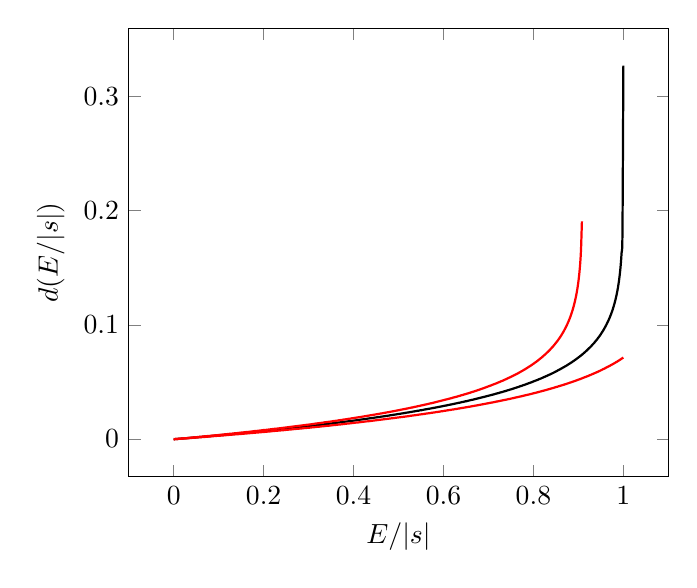
\begin{tikzpicture}
\begin{axis}[
    ylabel={$d(E/|s|)$},
    xlabel={$E / |s|$},
    trig format plots = rad,
    samples     = 500,
    domain      = 0:1,
    no markers, smooth]
  \addplot[name path=f1, black, thick] {(1 - (1 - x)^(1/31))};
  \addplot[name path=f1, red, thick] {(1 - (1 - x*1.1)^(1/31))};
  \addplot[name path=f1, red, thick] {(1 - (1 - x*0.9)^(1/31))};
  %\addplot[name path=f1, red, thick] {(1 - x)^((1/31) - 1))};
\end{axis}
\end{tikzpicture}
\caption{A plot of the function $d(E/|s|)$ with $k = 31$ in black. The red curves simulate the effect of an error of $\pm 10\%$ when measuring $E$.}\label{nfunc}
\end{figure}

\subsection{Embedding of $d$ in taxonomy trees}

We want to apply $d$ to a node $n$ in the context of a taxonomy tree such as in Figure \ref{simplerefdb}. More precisely, we estimate $d_n$ to be the maximum evolutionary distance \emph{from $n$'s parent to the data taxa\footnote{See Section~\ref{intrinsicqms} for the definition of the term \enquote{data taxon}.} under $n$}:
\begin{itemize}
\item
For that, $above(n)$ shall sum over the $k$-mers assigned to nodes above $n$ towards the tree's root excluding $n$. 
\item 
Regarding $below(n)$, we consider each path starting from $n$ to any leaf node under $n$ including $n$ itself. We sum over the $k$-mers assigned to all nodes along each path and set $below(n)$ to be the maximum sum from such paths. $p_n$ denotes some path leading to the maximum sum of $below(n)$. 
\end{itemize}
We set $d_n := d(E_n/|s_n|)$ by letting $E_n := below(n)$ and $|s_n| := above(n) + below(n)$.
This way, $d_n$ measures the evolutionary distance from $n$'s parent to the leaf of $p_n$. 
Since we use the maximum sum in $below(n)$, this estimate is conservative for $n$.
However, to depict evolutionary distances in a given taxonomy tree we must represent the portion $dp_n$ of $d_n$ relating to the branch from a node $n$'s parent to $n$ itself.
Let $c$ be the child of $n$ on the path $p_n$. It can be shown that $d_n \geq d_c$,\footnote{$E_n = below(n) = k_n + below(c) = k_n + E_c \geq E_c$ (where $k_n \geq 0$ is the number of $k$-mers stored at $n$ itself), while $|s_n| = above(n) + below(n) = above(n) + k_n + E_c = above(c) + below(c) = |s_c|$, so $E_n/|s_n| \geq E_c/|s_c|$, and therefore $d_n \geq d_c$ by monotonicity of $d$.} so we simply set $dp_n := d_n - d_{c}\geq 0$.

Figure \ref{simplerefdbdist} depicts a resulting taxonomy tree for the same database as in Figure \ref{simplerefdb} but with horizontal line lengths encoding distance portions.\footnote{We configuratively set the horizontal line lengths of the highest ranked nodes to a minimum although their $dp_n$ might be large. This is because the resulting distance portion is too unreliable and tends to cause a large but non-informative indentation in the tree. In Figure \ref{simplerefdbdist}, this exception affects the node \enquote{Viruses (10239) acellular root} only.}

  \begin{figure}[h]%
        \centering
\dbfig[width=12.95cm]{results/orthopox3_ftsvgtaxtree}
         \caption{Tree representation of a Genestrip $k$-mer database including three Orthopoxvirus species. The database is in the state \emph{right after the refinement} as in Figure \ref{ftsketch} (4). The tree depicts the same database as in Figure \ref{simplerefdb} but here, the length of a horizontal line to a node $n$ encodes the evolutionary distance portion $dp_n$. Both $d_n$ and $dp_n$ are also printed in brackets. The reddened lines indicate the branch for the $p_n$ starting from node $n$.
% Dashed lines signal less reliable evolutionary distances $d_n > t_n := 0.8$.
 }\label{simplerefdbdist}
    \end{figure}

The relatively compact depiction of taxonomy trees such as in Figure \ref{simplerefdbdist} allows for combining many species or even genera in a single representation and enables a fine-grained \emph{mapping of evolutionary relationships}. Hereby, the refinements resulting from Genestrip-FT integrate into the established NCBI taxonomy tree and support the visual display of the evolutionary distance $d$ via horizontal indentations. Figure \ref{borr_map} exemplifies this kind of mapping on a slightly larger scale with regard to the genus Borrelia (138).\footnote{The generation of such a map can be executed as a goal included by standard in Genestrip-FT. A resulting SVG file may be generated for any refined and unrefined Genestrip database.}
            
  \begin{figure}[h]%
        \centering
\dbfig[width=13cm]{results/borrelia_ftsvgtaxtree}
         \caption{Example of a phylogenetic mapping for the genus Borrelia (138) via a refined taxonomic tree with evolutionary distances included. The presentation approach is the same as in Figure \ref{simplerefdbdist}}\label{borr_map}
    \end{figure}

\section{Evolutionary distance distribution}

\subsection{Posterior distribution for the evolutionary distance}

We derive the probability distribution of $d$ given the observed count $E$ of differing unique $k$-mers, using Bayes' theorem. Let $N := |s|-k+1$ be the number of $k$-mers in $s$. We adopt a uniform prior $\pi(d) = 1$ on $d\in[0,1]$, reflecting no preference for any particular mutation rate. The binomial model from above gives the likelihood
\[
  P(E \mid d) = \binom{N}{E}\,p(d)^E\,[1-p(d)]^{N-E}, \qquad p(d) = 1-(1-d)^k.
\]
By Bayes' theorem the posterior satisfies
\[
  P(d \mid E) \;\propto\; [1-(1-d)^k]^E\,(1-d)^{k(N-E)}.
\]
To identify the normalising constant we substitute $v := (1-d)^k$, so $d = 1-v^{1/k}$ and $\mathrm{d}d = \frac{1}{k}\,v^{1/k-1}\,\mathrm{d}v$. The posterior density in $v$ becomes
\[
  P(v \mid E) \;\propto\; v^{\,N-E+\frac{1}{k}-1}(1-v)^{E},
\]
which is recognised as a $\mathrm{Beta}\!\left(N-E+\tfrac{1}{k},\;E+1\right)$ density. Hence the normalised posterior for $d$ is
\begin{equation}
  P(d \mid E) \;=\;
  \frac{k\,(1-d)^{k(N-E)}\bigl[1-(1-d)^k\bigr]^E}
       {B\!\left(N-E+\tfrac{1}{k},\;E+1\right)},
  \qquad d\in[0,1].
  \label{eq:dposterior}
\end{equation}

\subsection{Posterior mean and variance}

Since $d = 1-v^{1/k}$ with $v\sim\mathrm{Beta}\!\left(N-E+\tfrac{1}{k},\,E+1\right)$, and the $t$-th moment of a $\mathrm{Beta}(\alpha,\beta)$ variable equals $B(\alpha+t,\beta)/B(\alpha,\beta)$, the posterior mean is
\begin{equation}
  E[d\mid E] \;=\; 1 \;-\;
  \frac{B\!\left(N-E+\tfrac{2}{k},\;E+1\right)}
       {B\!\left(N-E+\tfrac{1}{k},\;E+1\right)}.
  \label{eq:dpostmean}
\end{equation}
For the variance we use $\mathrm{Var}(d\mid E) = \mathrm{Var}(v^{1/k}\mid E) = E[v^{2/k}\mid E]-(E[v^{1/k}\mid E])^2$, giving
\begin{equation}
  \mathrm{Var}(d\mid E) \;=\;
  \frac{B\!\left(N-E+\tfrac{3}{k},\;E+1\right)}
       {B\!\left(N-E+\tfrac{1}{k},\;E+1\right)}
  \;-\;
  \left(\frac{B\!\left(N-E+\tfrac{2}{k},\;E+1\right)}
             {B\!\left(N-E+\tfrac{1}{k},\;E+1\right)}\right)^{\!2}.
  \label{eq:dpostvar}
\end{equation}

\subsection{Delta method approximation for large $|s|$}

For genomic sequences $|s|$ is in the millions, so the posterior concentrates tightly around the point estimate $\hat{d} = d(E/|s|) = 1-(1-E/|s|)^{1/k}$ from Eq.~\eqref{distanceapprox}. Setting $\hat{v} = (1-\hat{d})^k$, the posterior variance of $v$ is approximately $\mathrm{Var}(v\mid E)\approx \hat{v}(1-\hat{v})/|s|$. Applying the delta method to $d = g(v) = 1-v^{1/k}$ with $g'(v) = -\tfrac{1}{k}\,v^{1/k-1}$ yields
\begin{equation}
  \mathrm{Var}(d\mid E) \;\approx\;
  \frac{(1-\hat{d})^{2-k}\bigl[1-(1-\hat{d})^k\bigr]}{k^2\,|s|}.
  \label{eq:ddeltavar}
\end{equation}
An approximate $\pm 1\sigma$ credible interval for $d$ is therefore $\hat{d}\,\pm\,\sqrt{\mathrm{Var}(d\mid E)}$. The bands are tight for moderate $E/|s|$ but widen rapidly as $E$ approaches $|s|$, confirming that the estimate becomes unreliable in that regime.

\iffalse
\begin{figure}[h]
\centering
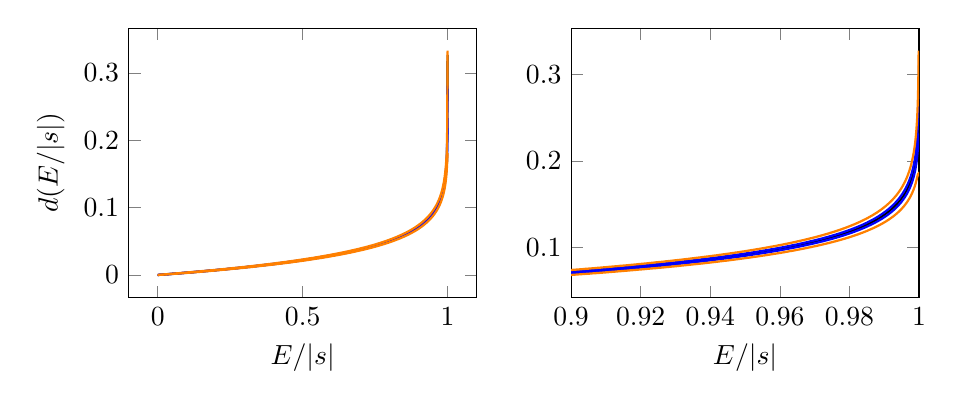
\begin{tikzpicture}
\begin{axis}[
    name=sigfull,
    ylabel={$d(E/|s|)$},
    xlabel={$E / |s|$},
    height=5cm, width=6cm,
    samples=500, domain=0:1,
    no markers, smooth]
  \addplot[black, thick] {(1 - (1-x)^(1/31))};
  \addplot[blue, thick, domain=0:0.9999] {(1-(1-x)^(1/31)) + x^0.5*(1-x)^(-29/62)/3100};
  \addplot[blue, thick, domain=0:0.9999] {(1-(1-x)^(1/31)) - x^0.5*(1-x)^(-29/62)/3100};
  \addplot[orange, thick, domain=0:0.9999] {(1-(1-x)^(1/31)) + x^0.5*(1-x)^(-29/62)/980};
  \addplot[orange, thick, domain=0:0.9999] {(1-(1-x)^(1/31)) - x^0.5*(1-x)^(-29/62)/980};
\end{axis}
\begin{axis}[
    at={(sigfull.east)}, anchor=west, xshift=1.2cm,
    xlabel={$E / |s|$},
    xmin=0.9, xmax=1,
    height=5cm, width=6cm,
    samples=2000,
    no markers]
  \addplot[black, thick, domain=0.9:1] {(1 - (1-x)^(1/31))};
  \addplot[blue, thick, domain=0.9:0.9999] {(1-(1-x)^(1/31)) + x^0.5*(1-x)^(-29/62)/3100};
  \addplot[blue, thick, domain=0.9:0.9999] {(1-(1-x)^(1/31)) - x^0.5*(1-x)^(-29/62)/3100};
  \addplot[orange, thick, domain=0.9:0.9999] {(1-(1-x)^(1/31)) + x^0.5*(1-x)^(-29/62)/980};
  \addplot[orange, thick, domain=0.9:0.9999] {(1-(1-x)^(1/31)) - x^0.5*(1-x)^(-29/62)/980};
\end{axis}
\end{tikzpicture}
\caption{Left: $\hat{d}\pm\sigma_d$ from Eq.~\eqref{eq:ddeltavar} with $k=31$ (black: $d(E/|s|)$; blue: $|s|=10^4$; orange: $|s|=10^3$). Right: zoomed view of $E/|s|\in[0.9,1]$ showing the bands widening as $E$ approaches $|s|$.}\label{nfuncsigma}
\end{figure}
\fi

   \section{Application to phylogeny}

    \subsection{Node precision for taxonomy improvements}

\todo{Internal note in the source below: what the refreshed subtree precisions do and do not say about this section, and the validation it would take to settle it.}

%
% ---------------------------------------------------------------------------------------------
% INTERNAL NOTE (added 2026-08-05) -- NOT FOR SUBMISSION AS IT STANDS.
%
% Do the numbers of Table \ref{dbsp} support using these measures for phylogeny? Partly, and not in
% the way the absolute values suggest.
%
% What speaks for it. Low values are rare and concentrated rather than scattered, which is the shape
% a usable flag would have. Over the 3,161 viral genera that hold k-mers the median sp in the
% refined database is exactly 1.0000; only 127 fall below 0.9 and none below 0.5. The tail is short
% and carries real mass rather than looking like noise:
%
%   Tequatrovirus   sp = 0.5352   (1,624,769 k-mers)
%   Cheoctovirus    sp = 0.5452   (  764,030 k-mers)
%   Pbunavirus      sp = 0.5929   (  505,574 k-mers)
%
% All three are phage genera. Whether that is a signal about their taxonomy or a property of phage
% taxonomy being unsettled to begin with is precisely the open question -- it is the first thing to
% look at, since a known-contentious group scoring low would be the cheapest possible evidence.
%
% What does not follow. A high average says flaws are rare; it does not say that a low value is
% *specific* to a structural flaw, which is what this section needs. Three confounders produce low
% values with no taxonomic meaning at all, and the first two grew with the move to all genomes:
%
%   - Incomplete genomes. Section \ref{nodeprecision} already notes that np deteriorates when the
%     genomes under a node are incomplete. Draft assemblies now dominate the eukaryotic databases.
%     This is why the sentence below prescribes complete genomes only, and it means the phylogeny
%     application needs its own database build rather than the one the rest of the paper uses.
%   - Contaminated assemblies. Lokmer et al. cite estimates of 1-30 % of nucleotides being of
%     bacterial or archaeal origin in the available Blastocystis genomes; such sequence distorts
%     c(a) directly.
%   - Bloom filter noise, measured here at the order of 1e-3 -- the same order as some of the
%     deviations one would want to interpret (see the footnote to Table \ref{dbsp}).
%
% How to settle it. Build a complete-genomes-only database, take a set of genera whose taxonomy was
% independently revised in recent years, and show that low sp discriminates them from the cases that
% missing or contaminated data explains. Until that discrimination is demonstrated the measure
% flags something real but unidentified, which is the reason this material sits in the appendix.
%
% One caveat that applies to reading Table \ref{dbsp} at all, phylogeny or not: after the leaf
% transformation every k-mer at a data taxon has |D| = 1 and hence p(a) = 1 by construction, so
% sp is bounded below by the share of k-mers stored at data taxa -- 99.4 % for parasites, 87.1 %
% for protozoa, 84.1 % for cv, 61.7 % for tb. The absolute values are therefore mostly bookkeeping;
% the refinement's *gain*, and tb where a real majority of the mass is at stake, are the informative
% parts.
% ---------------------------------------------------------------------------------------------
%
    Using a refined database with its refined taxonomy and with complete genomes only, low node precision allows for spotting potential structural flaws in the original, unrefined taxonomy. Figure \ref{npflaw} presents a basic example to highlight this use case:
    In (1), $X$ and $Y$ are not placed under the same node, even though their genomes are \emph{identical}. This causes a lowered node precision at their lowest common ancestor $W$.
    After correcting the taxonomy, node precision in (4) ends up being $1$ for every node that stores $k$-mers.

%The example from Figure \ref{npflaw} can be generalized: When the nodes of two data taxa, like $X$ and $Y$ from above, are falsely \emph{not} close enough together in the taxonomy, this \emph{always} manifests itself in a lowered node precision at \emph{their lowest common ancestor} $W$.
%This is because the LCA update will move every joint $k$-mer $a$ from $X$ and $Y$ to $W$ but the refinement must keep it there to maintain a path recall of $1$ for both.
%With $X$ and $Y$ being apart, this implies that another data taxon $Z$ exists near $X$ or $Y$ that does not contain $a$, therefore driving down $W$'s node precision.

    \begin{figure}[h]%
        \centering
        \small
        \begin{minipage}[c]{0.25\textwidth}
            \begin{flushleft}(1) Given $k = 2$ and $X$, $Y$, $Z$ under $W$ with associated sequences:\\
                $X$: \texttt{CCT}, $Y$: \texttt{CCT}, $Z$: \texttt{GCA}\\
                Here, the taxonomy groups $X$ and $Z$ under the intermediate node $V$.
            \end{flushleft}
        \end{minipage}
        \begin{minipage}[c]{0.2\textwidth}
            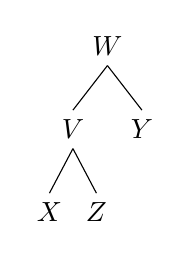
\begin{tikzpicture}
                \tikzset{every tree node/.style={align=center,anchor=north}}
                \Tree [.$W$ [.$V$ $X$ $Z$ ] $Y$ ]
            \end{tikzpicture}
        \end{minipage}
        \begin{minipage}[c]{0.25\textwidth}
            \begin{flushleft}(2) After the LCA update: \texttt{CC} and \texttt{CT} occur in both $X$ and $Y$ and so they move up to $W$. With $|D_W| = 3$, $|A_W| = 2$ and $c(\texttt{CC}) = c(\texttt{CT}) = 2$, this yields $np(W) = 2/3 < 1$.
            \end{flushleft}
        \end{minipage}
        \begin{minipage}[c]{0.2\textwidth}
            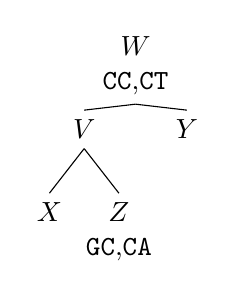
\begin{tikzpicture}
                \tikzset{every tree node/.style={align=center,anchor=north}}
                \Tree [.{$W$\\\texttt{CC},\texttt{CT}} [.$V$ $X$ {$Z$\\\texttt{GC},\texttt{CA}} ] $Y$ ]
            \end{tikzpicture}
        \end{minipage}

        \vspace{0.2cm}

        \begin{minipage}[c]{0.25\textwidth}
            \begin{flushleft}(3) The lowered $np(W)$ suggests that $Y$ rather than $Z$ belongs next to $X$. Correcting the taxonomy accordingly groups $X$ and $Y$ under $V$.
            \end{flushleft}
        \end{minipage}
        \begin{minipage}[c]{0.2\textwidth}
            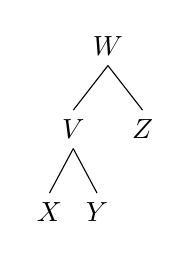
\begin{tikzpicture}
                \tikzset{every tree node/.style={align=center,anchor=north}}
                \Tree [.$W$ [.$V$ $X$ $Y$ ] $Z$ ]
            \end{tikzpicture}
        \end{minipage}
        \begin{minipage}[c]{0.25\textwidth}
            \begin{flushleft}(4) The resulting database with the \emph{corrected} tree and $2$-mers assigned accordingly: \texttt{CC} and \texttt{CT} now reside at $V$ and $np(n) = 1$ holds for every node $n$ that stores $k$-mers.\end{flushleft}
        \end{minipage}
        \begin{minipage}[c]{0.2\textwidth}
            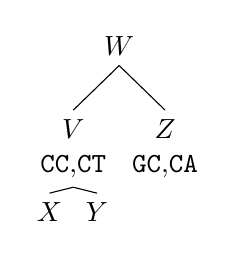
\begin{tikzpicture}
                \tikzset{every tree node/.style={align=center,anchor=north}}
                \Tree [.$W$ [.{$V$\\\texttt{CC},\texttt{CT}} $X$ $Y$ ] {$Z$\\ \texttt{GC},\texttt{CA}} ]
            \end{tikzpicture}
        \end{minipage}

        \vspace{0.2cm}

        \caption{Using node precision to spot a structural flaw in a taxonomy. In (2), $np(W) = 2/3$ lies below one, which indicates that the intermediate node $V$ groups the wrong data taxa. The corrected taxonomy in (3) yields $np(n) = 1$ for all $k$-mer-storing nodes in (4).}\label{npflaw}
    \end{figure}

  \section{Validation against other tools}
    
 
% like so: $d(E_n / k_n)$. But unfortunately, the following does not hold: $d_n(E_n/l_n) \neq \sum_i d_{n_i}(E_i/k_i)$.

    \subsection{Comparison with established phylogeny trees}
    
    Example candidates: Borrelia, Babesia, Malaria, Orthopoxvirus



\clearpage

\bibliography{sn-bibliography}

\end{document}
